% Computation Flow Reference for EP5GD00A (2012 Subaru Impreza FB20, Denso SH7058)
% Skeleton draft - 2026-10-18
% STATUS: exploratory, unverified. No table has been validated on hardware.
% Modeled on the Saab Trionic 7 Technical Reference (etnoy/t7ref) structure.
\documentclass[11pt,a4paper]{book}

\usepackage[utf8]{inputenc}
\usepackage{amsmath,amssymb}
\usepackage{tikz}
\usetikzlibrary{shapes,arrows,positioning}
\usepackage{hyperref}
\usepackage{booktabs}

\tikzstyle{stage} = [rectangle, rounded corners, draw, minimum width=5cm,
    minimum height=1cm, text centered, font=\small]
\tikzstyle{arrow} = [thick,->,>=stealth]

\title{EP5GD00A Computation Flow Reference\\
\large 2012 Subaru Impreza 2.0i (FB20) --- Denso SH7058\\
\large Exploratory draft, unverified}
\author{Built from AI-assisted reverse engineering\\(zero hardware validation)}
\date{2026-10-18 --- v0.1 skeleton}

\begin{document}
\maketitle

% ---------------------------------------------------------------------------
\chapter*{Unverified Research Notice}
\addcontentsline{toc}{chapter}{Unverified Research Notice}

Everything in this document is exploratory and unverified. Table counts,
addresses, scalings, labels, identities, chain-stage order, and combination
formulas may be wrong. No table has been validated on real hardware. No ROM
has been flashed. Do not tune, flash, or make decisions based on this data
until it is independently verified.

Evidence tags used throughout:
\begin{itemize}
  \item \textbf{DISASSEMBLED} --- verified in disassembly of this ROM
  \item \textbf{ROM-VERIFIED} --- raw bytes read from this ROM, values match
  \item \textbf{REFERENCE-DERIVED} --- matches reference definitions, not proven
  \item \textbf{SHAPE-INFERENCE} --- data behaves like the phenomenon, code untraced
  \item \textbf{OPEN THREAD} --- unknown
\end{itemize}

% ---------------------------------------------------------------------------
\chapter{Introduction}

This document describes the \emph{computation} performed by the EP5GD00A ECU:
the order of operations and the tables feeding each stage of the fuel,
timing, and drive-by-wire chains. It is the companion to the table
\emph{reference} (the 763-table RomRaider definition, v0.6); the reference
says what the tables are, this document says what the ECU does with them.

\section{Conventions}

Flash addresses are given as ROM offsets (e.g.\ \texttt{0xD46E8}). The
definition uses \texttt{storageaddress} attributes in the same space.

\section{Relationship to the table reference}

Chain stages cite tables by ROM address. See the wiki page
\texttt{Computation-Flow.md} for the living version of this document.

% ---------------------------------------------------------------------------
\chapter{DBW Chain}

Torque-based throttle control: pedal $\rightarrow$ requested torque
$\rightarrow$ throttle plate position. Two steps; no ``Requested Torque Base''
table exists on this ECU (confirmed negative finding).

\begin{center}
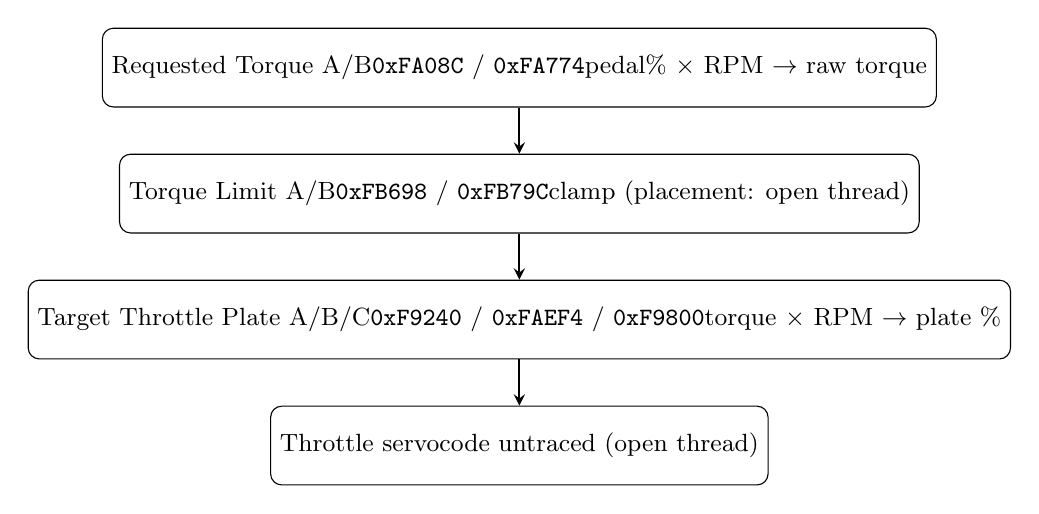
\begin{tikzpicture}[node distance=1.6cm]
  \node (s1) [stage] {Requested Torque A/B \\ \texttt{0xFA08C} / \texttt{0xFA774} \\ pedal\% $\times$ RPM $\rightarrow$ raw torque};
  \node (s2) [stage, below of=s1] {Torque Limit A/B \\ \texttt{0xFB698} / \texttt{0xFB79C} \\ clamp (placement: open thread)};
  \node (s3) [stage, below of=s2] {Target Throttle Plate A/B/C \\ \texttt{0xF9240} / \texttt{0xFAEF4} / \texttt{0xF9800} \\ torque $\times$ RPM $\rightarrow$ plate \%};
  \node (s4) [stage, below of=s3] {Throttle servo \\ code untraced (open thread)};
  \draw [arrow] (s1) -- (s2);
  \draw [arrow] (s2) -- (s3);
  \draw [arrow] (s3) -- (s4);
\end{tikzpicture}
\end{center}

\section{Stage 1: Requested Torque}

\texttt{0xFA08C} / \texttt{0xFA774}, $20\times18$ uint16BE,
scaling $x \cdot 0.0078125$ (raw torque units). X = accelerator pedal \%
(\texttt{0xF9FF4}, 0--100), Y = engine RPM (\texttt{0xFA044}, 1000--7010).
ROM-verified row 0: raw $[0, 9, 1636, 2991, \ldots] \rightarrow
[0.0, 0.07, 12.78, 23.37, \ldots]$.
Identical duplicates at \texttt{0xFA40C}/\texttt{0xFAAF4} are the leading
cruise/non-cruise hypothesis (open thread: selection logic).

\section{Stage 2: Torque limit}

\texttt{0xFB698} / \texttt{0xFB79C}, $10\times5$ float32BE.
Reference-derived. C/D variants searched for and not confirmed.

\section{Stage 3: Target Throttle Plate Position}

\texttt{0xF9240} (A, $50\times12$), \texttt{0xFAEF4} (B, $50\times12$),
\texttt{0xF9800} (C, $50\times19$). X = requested torque (5--187),
Y = RPM. Data scaling $x \cdot 0.002270655357 \rightarrow$ plate \%.
Each row carries a 2-u16 footer $[\texttt{0xB021}, X]$ with
\texttt{0xB021} $= 102.38\%$ max clamp (shape-inference).

\section{Limiters}

Rev limit (fuel cut) \texttt{0xCEA78} $= 6700.0$~RPM (ROM-verified float).
Speed-limiting throttle tables \texttt{0xF8E44}--\texttt{0xF8E68} use
increasing values $=$ progressive closure, not hysteresis.

% ---------------------------------------------------------------------------
\chapter{Fuel Chain}

\section{Stage order (hypothesis)}

\begin{enumerate}
  \item Air measurement: MAF scaling \texttt{0xDCEA0}, MAP scaling \texttt{0xDCCD8}
  \item Cylinder fill: VE families \texttt{0xC4E70} ($6\times11$, 42 tables)
        + \texttt{0xC6418} ($6\times18$, 42 tables), $x \cdot 0.00305175781$
  \item Base fuel: Primary Open Loop Fueling Non-Cruise \texttt{0xD46E8}
        ($10\times16$) / Cruise \texttt{0xD487C} ($10\times11$),
        $\mathrm{AFR} = 14.7 / (1 + x \cdot 0.0078125)$
  \item Closed-loop targets: CL Fueling Target Compensation A--D (load)
        \texttt{0xD34A6}/\texttt{0xD36F6}/\texttt{0xD3946}/\texttt{0xD3B96}
        ($11\times21$); ECT comp \texttt{0xC3FB0}
  \item Transient: tip-in tables + X-tau wall-wetting (see \S\ref{sec:xtau})
  \item Warmup/cranking: warmup enrichment \texttt{0xCF399},
        cranking IPW \texttt{0xCF586}/\texttt{0xCF5E6}/\texttt{0xCF646}
  \item CL$\leftrightarrow$OL transition: \texttt{0xD5180}/\texttt{0xD51D0}
  \item Decel: Idle Airflow Decel Adders \texttt{0xD9720}/\texttt{0xD9758}
        (rev hang mechanism)
  \item Final pulse width: injector latency near \texttt{0xD26A0};
        injector flow scalar \textbf{not found} (open thread)
\end{enumerate}

\section{Transient fueling and the X-tau model}
\label{sec:xtau}

Two mechanisms coexist; their relationship is the largest fuel-chain
open thread.

\paragraph{Pre-computed transient curves (shape-inference, high confidence).}
Wall-wetting fraction $X$ table \texttt{0xD319C} ($10\times9$, $x/32768$):
ROM-verified $0.615$ (idle, low load) $\rightarrow$ $0.050$ (high load),
monotonic in both axes --- textbook port wall-wetting.
The $8\times8$ cluster \texttt{0xD2864}--\texttt{0xD3024} uses
$X = [1..8]$ = engine cycles since transient: Table~10 at 1000~RPM reads
$[0.1187, 0.1187, 0.0500, 0.0250, 0.0125, \ldots]$, consecutive ratios
$\approx 0.5$ --- first-order exponential decay, the fuel-film evaporation
signature. Tables 4/5 \emph{rise} with $X$ (film accumulating onto walls).

\paragraph{Real-time filter (disassembled).}
Wall-wetting delta \texttt{0x36B1C} (RAM shift register \texttt{0x363DE}),
pair selection \texttt{0x365DC} (6 ECT tables \texttt{0xCF946}--\texttt{0xCF9E6}),
cycle counter \texttt{0x36640} (stops at 625 cycles, u16 \texttt{0xCE3D2}),
filter \texttt{0x36616} computing
\begin{equation}
  \mathrm{out} = (A \cdot B + C \cdot D + E \cdot F) \cdot G
\end{equation}

\paragraph{Rev hang.}
\texttt{0xD9720}/\texttt{0xD9758} (9-el, $x \cdot 0.001525879$~g/s,
X = vehicle speed): ROM-verified $[0.0, 0.0, 1.0, 1.75, \ldots]$~g/s.
The ECU adds idle airflow proportional to road speed when the throttle
closes --- this is the rev hang. DFCO tables were searched for and not
found (open thread).

% ---------------------------------------------------------------------------
\chapter{Timing Chain}

\section{Base timing}

\texttt{0xCC7A0} / \texttt{0xCCA88} ($13\times13$, $x \cdot 0.1$~$^\circ$BTDC):
ROM-verified raw $37$--$386 \rightarrow 3.7$--$38.6^\circ$
(idle $7.9^\circ$, cruise $17.3^\circ$, WOT $16.3^\circ$).
\texttt{0xCD670}/\texttt{0xCD778} ($7\times13$, X axis $[500..750]$
unidentified quantity --- open thread), \texttt{0xCCED4},
\texttt{0xCD010}, idle \texttt{0xD4640}.

\section{Knock control}

Knock Correction Advance Max A--E:
\texttt{0xCC450}/\texttt{0xCC2F6}/\texttt{0xCC638}/\texttt{0xCC6D8}/
\texttt{0xCC738}, scaling $x \cdot 0.01$.
ROM-verified A: raw $47$--$869 \rightarrow 0.47$--$8.69^\circ$;
ceiling largest at light-load/high-RPM, collapsing near zero at WOT.

Parameter cluster \texttt{0xD4A40}--\texttt{0xD4B50} (ROM-verified):
RPM hysteresis ranges \texttt{0xD4A5C} $[1100, 1200, 6900, 7000]$,
load pairs \texttt{0xD4AA4} $[0.48, 0.50]$, feedback retard limit
$-7.0^\circ$ (\texttt{0xD4A6C}), IAM initial $0.50$ (\texttt{0xD4AB8}),
step $0.03125$ (\texttt{0xD4AC0}).

Knock code: 31 functions \texttt{0x04B000}--\texttt{0x04C700}
(disassembled). Learned table in RAM \texttt{0xFFFF8800}/\texttt{0xFFFF8818},
initialized from flash \texttt{0xD4AC4}--\texttt{0xD4AD0} via
\texttt{0x4BB48}. Byte-wide \texttt{mov.b} refs to \texttt{0xFFFF87xx}
are on-chip peripheral registers --- dedicated knock DSP unit hypothesis
(open thread).

Working hypothesis for the combination (Subaru-standard, reference-derived,
\emph{not} traced in this ROM):
\begin{equation}
  \theta_{\mathrm{final}} = (\theta_{\mathrm{KCmax}} \cdot \mathrm{IAM})
    + \theta_{\mathrm{feedback}} + \theta_{\mathrm{fine}}
\end{equation}

\section{Dwell and AVCS}

Exactly one ignition dwell table \texttt{0xDD4C4} ($16\times5$,
RPM $\times$ battery volts) --- proven by all nine reference definitions
carrying exactly one. AVCS: four main cam-target maps
\texttt{0xC1650}--\texttt{0xC1D28}.

% ---------------------------------------------------------------------------
\chapter{Diagnostics: SSM}

SSM dispatcher \texttt{0x65380} (disassembled): handler table base
\texttt{0x6EFBC}, PID from \texttt{[GBR+0]}, \texttt{jsr @r2}.
Control block \texttt{0xFFFF9464}. Observation path, not control flow.
Parameter inventory is an open thread.

% ---------------------------------------------------------------------------
\appendix
\chapter{Open Threads}

\begin{enumerate}
  \item Final fuel summation order (base $\times$ warmup $\times$ tip-in
        $\times$ X-tau $\times$ CL trim --- additive? multiplicative? order?)
  \item Relation of pre-computed $8\times8$ transient tables to the
        real-time X-tau filter code (\texttt{0x36616})
  \item Injector flow scalar --- location or computation method
  \item DFCO tables (resume threshold, cut counters, enrichment singles)
  \item Actual knock/timing summation code in ROM
  \item DBW servo control loop; A/B/C variant selection
  \item VE 42-variant selection logic
  \item Base-timing C/D X-axis quantity $[500..750]$
  \item Knock DSP unit hypothesis (\texttt{0xFFFF87xx} peripherals)
  \item Cruise/non-cruise variant assignment across chains
\end{enumerate}

% ---------------------------------------------------------------------------
\chapter{Changelog}

\begin{tabular}{llp{9cm}}
\toprule
Date & Version & Change \\
\midrule
2026-10-18 & 0.1 & Skeleton: DBW, fuel, timing chains; TikZ flow for DBW;
                    X-tau filter equation; open-threads appendix. \\
\bottomrule
\end{tabular}

\end{document}
